\section{Overcoming the Pauli objection by weakening the requirements}

For several decades, Pauli's argument had prevented most theoretical attempts at
defining a self-adjoint time operator with the required commutation and uncertainty properties.
However, some research effort has been invested
into weakening some of those requirements, thus
introducing a notion of a time observable that did not satisfy
Pauli's ---explicit or implicit--- assumptions in the first place.

Notable examples of possible approaches involve:
renouncing the Hermiticity of the operator~$\hat{T}$ (replacing it with a more general symmetric operator);
allowing for the corresponding spectral measurement not to be projective (replacing it with a POVM);
or including the case of an \emph{imaginary} potential in the Hamiltonian,
to model absorption by a detector via loss of normalization (non-unitary evolution).

\subsection{Aharonov--Bohm}

In their 1961 paper, Aharonov and Bohm \parencite{AharonovBohm}
shown that ``energy can be measured
  reproducibly in an arbitrarily short time'',
thus apparently contradicting the time--energy indeterminacy theorized
by Mandelstam--Tamm (see also Sec. \ref{sec:T--H}) and by other authors.
It is worth observing,
as they do in the article, that in the Mandelstam--Tamm derivation time has a different meaning:
it is essentially the lifetime of a system in a particular state
and not the duration of the energy measurement process.
They also critically reviewed previous works by Landau and Peierls \parencite{LandauPeierls}
and by Fock and Krylov \parencite{FockKrylov}, discussed their level of generality and provided
counterexamples to their formulation of the time--energy uncertainty relation.

In their model, they considered a free particle as a ``clock''
and quantize (by symmetrizing the corresponding operators)
the classical relation
$t = y / v = m y / p$
for a particle that is at position $y = 0$ at time $t = 0$ and travels at velocity $v$ along the $y$ axis.
The corresponding time operator has then expression:
\begin{equation}
  \hat{T}_{AB} = \frac{m}{2} \qty( \hat{Y} \frac{1}{\hat{P}_y} + \frac{1}{\hat{P}_y} \hat{Y} ) \,\text{.}
\end{equation}
Such operator is claimed to be Hermitian, although with a singularity for $p_{y} = 0$.\footnote{
  This is stressed in a footnote of Aharonov--Bohm's paper.
  The reader might have noticed the irony of fundamental historical papers
  relegating important information at the level of footnotes
  ---and the present work, in many parts, not even trying to ``improve'' such a traditional trend.
}
With some simple algebra, a commutation relation $[\hat{H}_{c}, \hat{T}_{AB}] = \hbar/2$
can be proved, where $\hat{H}_c = \hat{P}_y^2/2m$ is the Hamiltonian of the free particle that is used as a ``clock''.

This seems to contradict Pauli's argument: however, more recent studies
\parencite{MugaAB98, MugaAB99, MugaAB99Err}
have shown that
$\hat{T}_{AB}$ is not, strictly speaking, self-adjoint but ``only'' maximally symmetric
(a weaker and more general condition).
An analogy has been made therein with the momentum on the half-line,
a restriction of the well known momentum operator to a subdomain
that is defined as
$\qty{\psi \in \mathscr{L}^2(\mathbb{R}): \psi(x) = 0 \; \forall x < 0}$ in position representation.
% Removal suggested due to mathematical intricacies...
% As opposed to the momentum in the half-line, $\hat{T}_{AB}$ does not have a self-adjoint extension though.
It has also been shown that the associated spectral measure is not projector valued, but
positive-operator valued (POVM). Projectors are a particular subclass of \term{positive operators}.
Among other applications, suitable positive operators can be used to extend von Neumann decomposition
in order to describe
open quantum systems and ``unsharp'' measurements.
Chapter~\ref{ch:decohere} will treat POVMs in detail and introduce the necessary
theoretical background.

Another apparent contradiction is the commutator $[\hat{H}_{c}, \hat{T}_{AB}] = \hbar/2$
---and the consequent uncertainty relation---
with Aharonov--Bohm's conclusion that
energy can be measured, in principle, with arbitrary precision in an arbitrarily short time;
but it should be noted that $\hat{H}_{c}$ is the energy of the clock, not of the system under energy-measurement,
thus the contradiction does not hold.

The Aharonov--Bohm model explicitly includes a clock in the description, i.e.,
a different system to the one under measurement;
and this separate system has one of its observables
on a well known dependency upon time, so the corresponding eigenvalues can be seen
as possible positions of the ``hand'' of the clock.
Aharonov and Bohm infer that $\hat{T}_{AB}$ must commute with all the observables
of the main system (and in particular the Hamiltonian, let's call it $\hat{H}_S$),
given that they are defined in different Hilbert spaces:
therefore, there is no
fundamental reason why the system energy represented by $\hat{H}_S$, and the clock time $\hat{T}_{AB}$,
could not have, in the same measurement,
arbitrarily
narrow statistical distributions around some of their eigenvalues.

This idea of a quantum description of time through modeling a ``clock''
(in other words, the notion of time as ``what is shown on a clock'' with some suitable properties)
has a certain historical relevance in that later models, independently developed,
have been based on that idea too.
In particular, we can mention
the Page--Wooters model (1983), where a peculiar relation is in place between the clock and the system,
of which we will not explore the details at this stage though,
as those will be discussed extensively (with numerical applications, experiments, and comparisons with other models)
from Chapter \ref{ch:pw} on.

\subsection{The papers by Allcock and following developments}

With three papers dated 1969 \parencite{Allcock-1, Allcock-2, Allcock-3}, G. R. Allcock
introduced a time-of-arrival quantum observable,
along with a first formulation of a detector model based on a non-Hermitian
Hamiltonian (by including a \term{complex potential}).
See in particular \cite[sec.II-IV]{Allcock-2}, where an anti-Hermitian term
$-iV_0\theta(x)$ is introduced in the Hamiltonian,
to model an absorber aimed at detecting
the arrival of a particle in the region $x>0$
(here $\theta$ is the Heaviside \term{step function}).
The particle state evolves
in non-unitary manner, with a transfer of probability
from an ``incident channel''
into ``orthogonal and time-labelled measurement channels''.
Unfortunately Allcock came to negative conclusions regarding this approach.
Among other objections, he noticed that when $V_0$ is large the particle is not absorbed but reflected;
while, when it's small (i.e. the detector has a low absorption rate), the particle is eventually absorbed but
with an indetermination $\delta_T \sim \frac{1}{2}V_{0}^{-1}$
that becomes, in such case, impractically large.
Also, Allcock did not directly tackle the Pauli objection
but rather maintained that argument.

The limitations of complex potentials either causing reflection
or not absorbing sufficiently have been resolved
in the following literature
by noting that the results by Allcock were not general, and
potentials can be constructed that absorb the whole wave packet
and avoid reflection \parencite{Muga_TOAQM, Muga_CompositeAbsPot, ComplexAbsPot}.

\subsubsection{How a complex potential emerges}

Among the methods to define a time-of-arrival quantum observable,
the detector model by Allcock
---including the following enhancements---
is an \emph{operational} one,
in that it models a measurement procedure \parencite[sec.9]{Leavens_TOA}
rather than focusing on constructing an operator that satisfies certain requirements
(like the Kijowski distribution, see for example \cite[sec.8]{Leavens_TOA}).

The introduction of complex potentials, a non-Hermitian Hamiltonian and
the non-unitary evolution (of a pure state!) may appear artificial to some,
and in contradiction with the fundamental rules of quantum mechanics.

\citereset
In fact, as pointed out well in \cite{Halliwell_Irreversible},
an \emph{effective} complex potential and the consequent loss of normalization
only emerge after ``tracing out'' a portion of the whole system,
which includes the particle, the detector and the environment altogether.
Such whole tripartite system \emph{is} closed, in a pure state, and evolves unitarily.
The particle wavefunction is also an ``effective'' one derived from its density operator.
(See also
  \cite{Wave-function_approach, Hegerfeldt_WignerSymposium, TheQuantumJumpApproach};
  \cite[Ch. 6]{TQM2};
and
  \cite[sec.6.7.1 ``Simulating Quantum Trajectories'']{WallsMilburn}).

Not surprisingly, absorption is an \term{irreverersible} process.

While a complex potential can be \emph{postulated} in order to obtain
phenomenological laws governing arrival times and detectors,
it can also be \emph{derived} from first principles and within the established framework
of open quantum systems, namely the master equation
for an irreversible detector.
The core ideas behind this derivation
can be ---very briefly--- summarized as follows.

The detector is modeled by a two-level system with $\ket{1}$ being the state of no-detection
and $\ket{0}$ the state of detection.
We also introduce the raising and lowering operators $\sigma_{+}=\ketbra{1}{0}$, $\sigma_{-}=\ketbra{0}{1}$.
The Hamiltonian of the detector is such to have $\ket{0}$
at a lower energy, so the detector ``decays'' when it ``clicks''. It's an irreversible transition because
of the coupling with the environment.
The Hamiltonian encompassing the particle, the detector, the environment and the interaction reads
\begin{equation}
  H = H_s + H_d + H_{E} + V(x)  H_{dE} \,\text{,}
\end{equation}
with $H_s$ being the Hamiltonian of a free particle and
\begin{subequations}\begin{align}
  H_d     &= \frac{1}{2}\hbar\omega \qty(\ketbra{1} - \ketbra{0}) \\
  H_{E}   &= \sum_n \hbar \omega_n a_n^{\dag} a_n \\
  H_{dE}  &= \sum_n \hbar \left( \kappa^*_n \sigma_{-} a_n^{\dag} + \kappa_n \sigma_{+} a_n \right) \\
  V(x)    &= \theta(-x) \,\text{,}
\end{align}\end{subequations}
where $a$ and $a^{\dagger}$ are the creation and annihilation operator for the electromagnetic field,
which constitutes the ``environment''; $V(x)$ is chosen to be a step function
i.e. the simplest function that makes the detector respond
when the particle reaches the region ($x<0$);
and the coupling constants $\kappa_{n}$ are to be intended in the same sense of the Jaynes--Cummings model
---in fact, the expressions of $H_d$ and $H_E$ also recall it
(\cite[sec.10.2]{WallsMilburn}, \cite{JCM} and many others).
This model essentially describes the detector as a Jaynes-Cummings atom
with the peculiarity that its coupling with the environment
is only activated by the position distribution
of another particle.

Tracing out the environment, and with some ``standard'' assumptions
(initial environment at zero temperature,
initial separable state ``undetected'' $\rho(0) = \ketbra{\psi_0}\ox\ketbra{1}$,
Markov approximation,
weak coupling),
the \emph{reduced} dynamics of the particle and the detector
is governed by the \emph{master equation}\footnote{
  Most details, calculation steps and possible generalizations are clearly skipped here, and can be found
  in the original article by J. J. Halliwell \parencite{Halliwell_Irreversible}
  and references therein.
}
\begin{equation}
  \dot{\rho} = -\frac{\iu}{\hbar} [ H_s + H_d, \rho] 
- { \gamma \over 2} \left( V^2 (x ) \sigma_{+} \sigma_{-}  \rho \ +  \rho
\sigma_{+} \sigma_{-}   V^2 (x)  \ -  \ 2 V (x) \sigma_{-}  \rho \sigma_{+} V (x )
\right)
\,\text{,}
\end{equation}
with $\gamma$ being ``a phenemonological constant determined by the distribution of oscillators in the
environment and underlying coupling constants'' \parencite{Halliwell_Irreversible}.

A general solution is in the form
\begin{equation}
  \rho =
  \rho_{11} \ox \ketbra{1}{1}
+ \rho_{01} \ox \ketbra{0}{1}
+ \rho_{10} \ox \ketbra{1}{0}
+ \rho_{00} \ox \ketbra{0}{0}
\,\text{,}
\end{equation}
with
\begin{subequations}\begin{align}
  \dot{\rho}_{11} =& -\frac{\iu}{\hbar} [ H_s, \rho_{11} ] -\frac{\gamma}{2}\left(V(x)\rho_{11} + \rho_{11}V(x)\right) \label{eq:drho11} \\
  \dot{\rho}_{01} =& -\frac{\iu}{\hbar} [ H_s, \rho_{01} ] -\frac{\gamma}{2}\rho_{01}V(x) + \iu \frac{\hbar\omega'}{2} \rho_{01}\\
  \dot{\rho}_{10} =& -\frac{\iu}{\hbar} [ H_s, \rho_{10} ] -\frac{\gamma}{2}V(x)\rho_{10} - \iu \frac{\hbar\omega'}{2} \rho_{10}\\
  \dot{\rho}_{00} =& -\frac{\iu}{\hbar} [ H_s, \rho_{00} ] +\gamma V(x)\rho_{11}V(x) \,\text{,}
\end{align}\end{subequations}
and $\omega'$ a ``renormalized'' value for the characteristic frequency $\omega$ in $H_d$.

Just to give an idea of how the complex potential emerges, let's now focus on $\rho_{11}$
and the corresponding probability of not being detected, which is
\begin{equation}\label{eq:p_nd}
  p_{nd} = \Tr \rho_{11}(\tau) = \int_{-\infty}^{\infty} \dd{x} \rho_{11}(x, x, \tau) \,\text{,}
\end{equation}
where $\rho_{11}(x, x, \tau)$
-- or, more generally, $\rho_{ij}(x, x, \tau)$ for each $i, j = 0, 1$ --
are (diagonal) density matrix elements such that, in general:
\begin{equation}
  \rho_{ij}(\tau) = \int_{-\infty}^{\infty} \dd{x_1} \int_{-\infty}^{\infty} \dd{x_2} \rho_{ij}(x_1, x_2, \tau) \ketbra{x_1}{x_2}
  \, \text{.}
\end{equation}

Now, the solution to the \eqref{eq:drho11} can be written
\begin{equation}\label{eq:rho11.evol}
  \rho_{11}(t) =  e^{-\frac{\iu}{\hbar}H_{s}t-\frac{\gamma}{2}Vt}
  \rho_{11}(0)    e^{ \frac{\iu}{\hbar}H_{s}t-\frac{\gamma}{2}Vt} \, \text{.}
\end{equation}
If $\rho_{11}$ were in a pure state, say $\rho_{11}(t) = \ketbra{\psi(t)}$
(the ``undetected wavefunction''),
and recalling that $\rho_{11}(0) = \ketbra{\psi_0}$,
eq. \eqref{eq:rho11.evol} can be reformulated as
\begin{equation}
  \ket{\psi(t)} =
  e^{-\frac{\iu}{\hbar}H_{s}t-\frac{\gamma}{2}Vt} \ket{\psi_0} =
  e^{-\frac{\iu}{\hbar} \qty( H_{s} -\iu\frac{\hbar}{2}\gamma V ) t} \ket{\psi_0} \,\text{,}
\end{equation}
showing that the particle evolves as if an ``imaginary'' (anti-Hermitian) term
$-\iu\frac{\hbar}{2}\gamma V$ was added to its otherwise free Hamiltonian $H_s$.
This ``proves'' the validity of the complex potential model as an \emph{effective} theory,
and the consistency
with the unitary evolution of the ``bigger picture'' quantum system.

Another consequence of treating $\rho_{11}$ as a pure state is that the probability of no detection
\eqref{eq:p_nd} can be expressed as
\begin{equation}
  p_{nd}(\tau) = \int_{-\infty}^{\infty} \dd{x} \qty|\psi(x, \tau)|^2 \, \text{,}
\end{equation}
which is the (non conserved) norm $\norm{\psi}$ of this effective state vector.
Therefore, the probability that the detection \emph{has} happened
up to time $\tau$, which is $1 - p_{nd}(\tau)$, is equal to the
\emph{loss of normalization} $1 - \norm{\psi}$ at that time.
This is the total probability that the detection has happened from the initial time
($t=0$ in our chosen settings)
to $t = \tau$. In terms of probability density (per unit of time)
$\mathbb{P}(t)$, it is therefore
\begin{equation}
  \mathbb{P}(t) = - \dv{\norm{\psi}}{t} \,\text{.}
\end{equation}

\subsection{Kijowski}\label{sec:kijowski}

In 1974, Jerzy Kijowski pursued an axiomatic approach towards a
time-of-arrival quantum distribution. In his paper \parencite{Kijowski}, he sought to compute
the probability distribution for a particle to intersect an hypersurface
$\mathcal{Q}$ immersed in the $(3+1)$-dimensional space-time.
Classically, the trajectory of a particle is a curve in this $3+1$ space
which intersects the hypersurface at a certain point $(\bar{t^{\vphantom{1em}}}, \bar{x^1}, \bar{x^2}, \bar{x^3})$.
An example of a purely
space-like hypersurface is defined by an equation like
$t=\bar{t}$ (which is, more specifically, an hyperplane).
The point coordinates
at which the particle passes through it
essentially tell \emph{where}
the particle is at time $\bar{t}$,
i.e. the values of $\bar{x^1}$, $\bar{x^2}$, $\bar{x^3}$,
given that $\bar{t}$ is known.
For a quantum particle, the exact coordinates $\bar{x^1}$, $\bar{x^2}$, $\bar{x^3}$
are replaced by a complex wavefunction $\psi_{\bar{t}} \in \mathscr{L}^2(\mathbb{R}^3)$
of the variables $x^1$, $x^2$, $x^3$,
where:
$\psi_{\bar{t}}(x^1, x^2, x^3) = \braket{x^1, x^2, x^3}{\psi_{\bar{t}}}$;
$\bra{x^1, x^2, x^3}$ is an eigenbra of the 3-dimensional position operator $\bra{x^1} \ox \bra{x^2} \ox \bra{x^3}$;
and $\ket{\psi_{\bar{t}}}$ is the state ket at time $\bar{t}$ in the ordinary quantum mechanics sense.

The probability that the particle hits this hyperplane at its point of coordinates $x^1, x^2, x^3$
is given by the square modulus $\abs{\psi_{\bar{t}}(x^1, x^2, x^3)}^2$.
More generally, probability distributions are given by bilinear functionals of the wavefunction.

Kijowski then considers an hypersurface that is spanned by one time-like vector and two independent
space-like vectors (as opposed to the purely space-like hypersurface mentioned above).
The time coordinate of the intersection with the \term{world line}
of a particle tells \emph{when} the particle traverses the surface.
(Again, in the quantum sense, such exact value shall be replaced by a probability distribution).
One obvious example would be the hyperplane $x^3 = \bar{x^3}$.
Or, more simply, $x^3 = 0$, which we will consider from now on.

Given all the above considerations, the first requirement is:
\begin{axiom}\label{ax:kijowski:first}
  The probability distribution for the time-of-arrival of a particle at a given surface
  is given by a continuous positive bilinear functional
  \begin{equation*}
    F[\psi_{t}] \eqbydef T_F[\psi_{t}, \psi_{t}] \, \text{.}
  \end{equation*}
\end{axiom}

The reader can classically and intuitively picture an horizontal plane,
a particle below it traveling upwards, and ask the question
``when does the particle pass through?''. The point of intersection,
besides the coordinate $\bar{x^3}$ which is known, and the other two space-like coordinates $\bar{x^1}$ and $\bar{x^2}$,
will have the time coordinate $\bar{t}$ which is the \term{time of arrival} at the hypersurface.

Consistently with the above, Kijowski initially restricted the study to
particles with positive momentum, which in terms of momentum wavefunction
obviously means ${\phi(p^1, p^2, p^3) = 0} \,\, {\forall \, p^3 < 0}$.

The momentum representation $\phi$ is, in fact, used the most in Kijowski's
paper, to make the theory explicit. The rest of this Section will reflect that.

Other requirements for the probability distribution $F[\phi_t]$ are
\begin{axiom}
  $F[\phi_t] \ge 0 \ \forall t$
\end{axiom}
\begin{axiom}
  If $\norm{\phi_t}_{\scriptscriptstyle{\mathscr{L}^2(\mathbb{R}^3)}} = 1 \ \forall t$, then $\int F[\phi_t] \dd t = 1$
\end{axiom}
\begin{axiom}
  $F[\pi(\phi)] = F[\phi]$.
\end{axiom}
In the last one, $\pi$
is the representation of any Galilei transformation
which preserves $\mathcal{Q}$
e.g. a translation which is parallel to the surface
(the first Kijowski paper considered the nonrelativistic case).

From now on, we will consider, for simplicity, the surface $x^3 = 0$.

For reasons of symmetry, in terms of time-of-arrival at $x^3 = 0$,
one intuitively expects a particle
``traveling upwards from the bottom'' to be equivalent
to a particle
``traveling downwards from the top'',
if both position and momentum have their sign flipped.
For a quantum wavefunction in the position representation,
this means
replacing $\psi(\va{x})$ with $\psi(-\va{x})$.
Or $\phi(\va{p})$ with $\phi^{*}(\va{p})$ in momentum representation:
\begin{axiom}
  $F[\phi^{*}_t] = F[\phi_t]$, $\forall t$.
\end{axiom}

The last requirement is that
\begin{axiom}\label{ax:kijowski:last}
    The \term{dispersion}, defined as
    \begin{equation}\label{eq:kijowski:dispersion}
      \int \dd{t} t^2 F[\phi_t] - \qty(\int \dd{t} t F[\phi_t] )^2 \text{,}
    \end{equation}
    is finite.
\end{axiom}

Given the above axioms, Kijowski proved the following
\begin{theorem}
  $\,$

  \begin{enumerate}
    \item
      A specific functional $F_0$ which minimizes the variance
      \eqref{eq:kijowski:dispersion}
      exists;
    \item
      The average value $\int \dd{t} t F[\phi_t] $ is constant over the class of
      functionals defined by the axioms;
    \item
      $F_0$ has the expression
      \begin{multline}\label{eq:kijowski_bilinear_full}
        F_0[\phi_t] = T_{F_0}[\phi_t, \phi_t] =
            \frac{1}{m(2\pi\hbar)^4}
            \int\displaylimits_{p_{3}', p_{3}'' \ge 0} \sqrt{p_{3}' p_{3}''} \phi_t^{*}(p_1, p_2, p_{3}') \phi_t(p_1, p_2, p_{3}'')
            \dd p_1 \dd p_2 \dd p_{3}' \dd p_{3}''
            = \\
                      \frac{1}{2 \pi m \hbar} \abs{\int_0^{\infty} \dd p \sqrt{p} e^{-\iu p^{2} t / 2m\hbar} \phi_{0}(p)}^2
                      \, \text{,}
      \end{multline}
  \end{enumerate}
  where the wavefunction is in the momentum representation and the free evolution
  $\phi_t(p) = e^{-\iu p^{2} t / 2m\hbar}\phi_{0}(p)$
  is assumed.
\end{theorem}

Please note that the bilinear $T_{F_0}[\phi_t, \phi_t]$ in the \eqref{eq:kijowski_bilinear_full}
is a particular case of $T_{F_0}[\phi'_t, \phi''_t]$, where $\phi' = \phi'' \eqbydef \phi$.

While this distribution is ``well behaved'' i.e. it has similar properties of other distributions
associated to quantum observables described by self-adjoint operator and projective measurement,
the corresponding operator found by Kijowski was not self-adjoint and the corresponding
operator-valued measure was not projective.
It was, more weakly, a \term{Positive Operator Valued Measure} or \term{POVM}.
See, for example, \cite[Sec. 10.3]{TQM1},
for a summary of POVMs, and Chapter \ref{ch:decohere}.

% Intermediate calculation for to obtain The Book's formulas from Kijowski paper.
%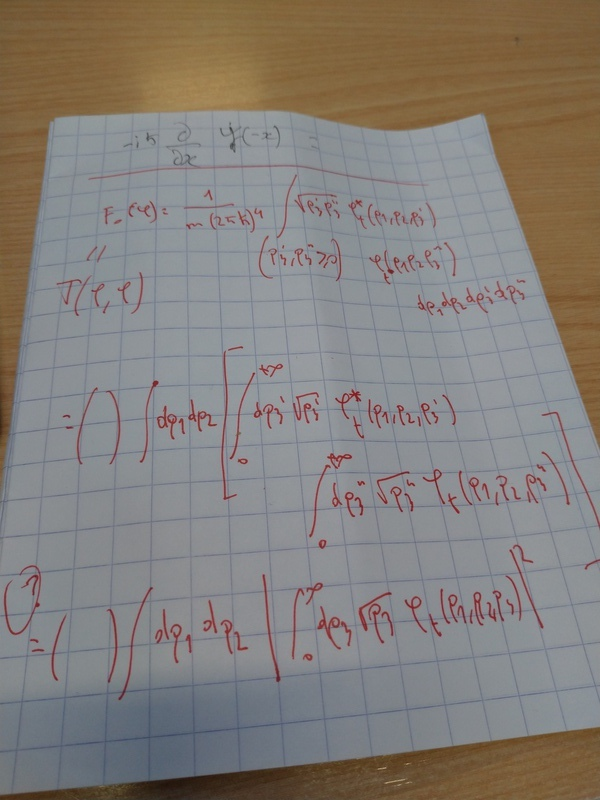
\includegraphics[width=\linewidth]{img/tmp/kijowski1.jpg}

\subsection*{TODO}

Detector model, Ch. 4 Vol. 2 book? \parencite[Ch. 4]{TQM2}.